\documentclass[aps,prl,twocolumn,superscriptaddress,nofootinbib,amsmath,amssymb]{revtex4-2}
\usepackage{graphicx}
\usepackage{xcolor}
\usepackage{amsthm}
\usepackage{bm}
\usepackage[colorlinks=true,linkcolor=blue!50!black,citecolor=blue!50!black,urlcolor=blue!50!black]{hyperref}

% ---------------------------------------------------------------------------------------------------
% SCOPE MACROS. The present draft covers vacuum solutions only.
% MATTER-SLOT (scope): if the extension to matter obeying the null energy condition is established,
% redefine \ScopeClass and \ScopeShort here and fill the MATTER-SLOT blocks below. Nothing else in the
% statements refers to the vacuum assumption except the positivity of the Liouville measures (see the
% MATTER-SLOT block in the mechanism paragraph and in the discussion).
\newcommand{\ScopeClass}{vacuum solutions of three-dimensional gravity with negative cosmological constant}
\newcommand{\ScopeShort}{vacuum}
% ---------------------------------------------------------------------------------------------------

\newtheorem{theorem}{Theorem}
\newtheorem{proposition}{Proposition}
\theoremstyle{definition}
\newtheorem*{remark}{Remark}

\newcommand{\AdS}{\mathrm{AdS}_3}
\newcommand{\Hyp}{\mathbb{H}^2}
\newcommand{\Cut}{\mathcal{C}}
\newcommand{\CN}{\mathcal{C}_N}
\newcommand{\eps}{\epsilon}
\newcommand{\SM}{Supplemental Material~\cite{SM}}

\begin{document}

\title{Time dependence does not enlarge the holographic entropy cone\\ in three-dimensional vacuum gravity}
% MATTER-SLOT (title): replace "vacuum gravity" if the result is extended to matter.

\author{Ansh Mishra}
\affiliation{[Affiliation placeholder]}
\author{Aryan Senthilkumar}
\affiliation{[Affiliation placeholder]}

\date{\today}

\begin{abstract}
In time-reflection-symmetric holographic states the Ryu--Takayanagi (RT) entropies obey the linear
inequalities of the holographic entropy cone. Whether time dependence allows the covariant
Hubeny--Rangamani--Takayanagi (HRT) entropies to leave this cone has been an open question. We settle it for
\ScopeShort{} three-dimensional gravity with negative cosmological constant, for every topology (rotating BTZ
black holes, rotating multiboundary wormholes, wormholes with handles) and arbitrary boundary regions: the HRT
entropy vector lies in the RT cone at every sufficiently small cutoff, and the closure of the covariant cone
equals the RT cone. The proof rests on an exact decomposition: the regulated HRT vector is a
cutoff-independent graph-model vector plus exactly one Bell-pair term per entangling point.
\end{abstract}

\maketitle

\emph{Introduction.}---%
In holography the entanglement entropy of a boundary region $A$ is the area of an extremal surface in the
bulk: the minimal surface on a time-symmetric slice (RT)~\cite{RyuTakayanagi2006}, or in general the
minimal extremal surface homologous to $A$ (HRT)~\cite{HRT2007}. Static RT entropies obey strong
subadditivity~\cite{HeadrickTakayanagi2007}, monogamy of mutual information (MMI)~\cite{HaydenHeadrickMaloney2013}
and infinitely many further linear inequalities, which together cut out the \emph{holographic entropy cone}
$\CN$ of $N$-party entropy vectors~\cite{Bao2015,HernandezCuenca2019,AvisHernandezCuenca2023}. These
inequalities are proved on a static slice, by cutting and pasting minimal surfaces, and are equivalently the
inequalities obeyed by min-cuts of weighted graphs~\cite{Bao2015}. Physically interesting states---black-hole
formation, quenches, rotating black holes---are not time-symmetric, and their entropies are given by HRT.
Strong subadditivity and MMI survive time dependence~\cite{Wall2014}, but whether the higher inequalities do
is open~\cite{GGHH2025,GrimaldiHeadrick2026}; approaches via maximin~\cite{Wall2014},
minimax~\cite{GGHHMinimax2025}, covariant bit threads~\cite{HeadrickHubeny2023} and covariant graph
models~\cite{Zhao2026} have not settled it. The question is whether dynamics can produce geometric
entanglement patterns that no static geometry produces.

In $2+1$ bulk dimensions Czech and Dong proved all contraction-map inequalities for simply connected bulks,
without restricting to vacuum, using a positive measure on kinematic space~\cite{CzechDong2019}. For multiply
connected bulks their universal-cover step fails: ``an infinite number of surfaces enter on both sides of the
inequality''~\cite{GGHH2025}. Grado-White, Grimaldi, Headrick and Hubeny (GGHH) gave an argument for
$\pi_1=\mathbb{Z}$, also with matter, which they do not claim to be fully rigorous and which the recent review
lists as a proof~\cite{GrimaldiHeadrick2026}; they explained why it does not extend to free groups, found no
violation in extensive numerical tests on vacuum multiboundary wormholes, and left the multiply connected case
open~\cite{GGHH2025}. This Letter settles the vacuum case.

\emph{Result.}---%
For all \ScopeClass{} of the class described below---any topology, any rotation---and every assignment of
$N$ parties to boundary intervals and whole asymptotic boundaries, the HRT entropy vector lies in $\CN$ for
every cutoff below an explicit threshold; every valid RT inequality holds, with a cutoff-independent slack if
it is balanced at the entangling points and a slack diverging to $+\infty$ otherwise; and the closure of the
set of covariant entropy rays is $\CN$. Time dependence does not enlarge the cone.
% MATTER-SLOT (result): if extended, state here the class "with matter obeying the NEC" and its hypotheses.

The HRT prescription is used in its standard form: a minimal extremal curve $\gamma$ anchored at $\partial A$,
with a homology region $R$, $\partial R=\gamma\cup A$, lying on a Cauchy slice of the conformally completed
spacetime~\cite{HHLR2014}. We show that the answer is the same whether the slice is only required to be
acausal (the convention of Ref.~\cite{HHLR2014}) or to be compact, smooth and uniformly spacelike. The
statements concern the leading classical term.

\emph{Setting.}---%
Locally $\AdS$ spacetimes are quotients of $\AdS=\mathrm{PSL}(2,\mathbb{R})$, with isometries
$x\mapsto g_L x g_R^{-1}$~\cite{BTZ1992,ABHP1996,ABH1999,Krasnov2000,SkenderisVanRees2011}. Let $S$ be an
oriented surface of finite type with boundary and $\rho_L,\rho_R$ two convex cocompact Fuchsian
representations of $\pi_1(S)\neq1$ with the same marking: holonomies of two hyperbolic structures
$X_L=\Hyp/\rho_L$ and $X_R=\Hyp/\rho_R$ with funnel ends. The group $\Gamma=\{(\rho_L(\gamma),\rho_R(\gamma))\}$
acts properly discontinuously on the invisible domain $\tilde D$ of its limit set, and $M=\tilde D/\Gamma$ is a vacuum
spacetime with one asymptotic region per funnel~\cite{Mess2007,Barbot2008,BKS2011,BonsanteSeppi2020}. This
covers rotating BTZ ($\pi_1=\mathbb{Z}$), rotating multiboundary wormholes and wormholes with handles. $M$ is
time-symmetric iff $X_L=X_R$; for $X_L\neq X_R$ and non-abelian $\pi_1$ it is not even stationary. Excluded
are extremal horizons (parabolic holonomy), conical defects and non-orientable quotients; global $\AdS$ is
covered by Ref.~\cite{CzechDong2019}.

A boundary Cauchy slice lifts to an acausal circle in $\partial\AdS=\mathbb{RP}^1\times\mathbb{RP}^1$, so
each boundary point has a left and a right coordinate, which are points of the ideal boundaries of $X_L$
and $X_R$. The endpoints of all regions form a finite set $P$ of marked points. A \emph{cut} for a region $A$ is
an embedded multicurve on $S$---closed curves and arcs ending at the points of $\partial A$, one end at each---that
bounds a region whose closure meets the ideal boundary exactly in $A$; $\Cut(A)$ is the set of cuts up to
isotopy. The closed spacetime geodesic in the class of $\gamma\in\pi_1(S)$ has length
$\tfrac12[\ell_L(\gamma)+\ell_R(\gamma)]$, the mean of the two chiral lengths, and the same holds for
regulated arcs with horocyclic cutoffs~\cite{GGHH2025,MazzoliViaggi2023,SM}. Figure~\ref{fig:wormhole}
illustrates a cut on the two chiral surfaces.

\begin{figure}[t]
\centering
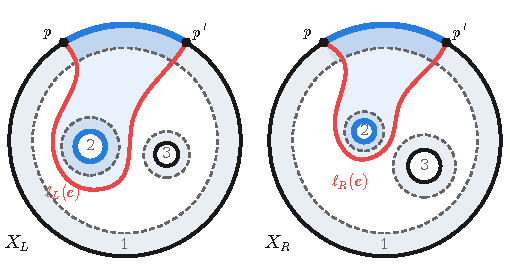
\includegraphics[width=\columnwidth]{fig/fig1_wormhole.pdf}
\caption{The two chiral surfaces $X_L$, $X_R$ of a rotating three-boundary wormhole (pairs of pants;
shaded annuli are funnels, dashed circles horizons, thick circles conformal boundaries). The region $A$
(blue) is an interval $[p,p']$ of boundary~1 together with all of boundary~2. One cut class $c$ (red),
an arc from $p$ to $p'$ around funnel~2, has different lengths on the two surfaces; the HRT curve of class
$c$ has length $\frac12[\ell_L(c)+\ell_R(c)]$, and the minimum is taken over classes common to both
surfaces.}
\label{fig:wormhole}
\end{figure}

\begin{theorem}[HRT as a common-class minimum]\label{thm:H}
For every region $A$ and every cutoff $\eps\le\eps_0$,
\begin{equation}\label{eq:H}
4G_N\,S^\eps(A)=F^\eps(A):=\min_{c\in\Cut(A)}\tfrac12\big[\ell^\eps_{X_L}(c)+\ell^\eps_{X_R}(c)\big],
\end{equation}
both when homology slices are only required to be acausal and when they are required to be compact, smooth
and uniformly spacelike; the minimum is attained in both classes.
\end{theorem}

GGHH already used the right-hand side of Eq.~\eqref{eq:H} as their working formula, with the homology
condition imposed combinatorially~\cite{GGHH2025}; Theorem~\ref{thm:H} derives it from the HRT prescription.
For ``$\ge$'', the components of an HRT candidate lift to disjoint arcs in a disc-like slice; their endpoints on
the lifted boundary curve are therefore unlinked, so they project to an embedded multicurve on $X_L$ and on $X_R$
in one common class, and a parity count reconstructs the homology region. For ``$\le$'', each cut class is
realised on an explicit slice: we fill $\Hyp$ by an invariant family of ideal triangles that contains the arcs of
the cut and spirals onto its closed geodesics, and replace each triangle by the totally geodesic ideal triangle
of $\AdS$ on the corresponding boundary points. A separation lemma---convex hulls of complementary arcs of an
acausal circle are spacelike separated---makes the union an acausal disc, a pleated surface of the kind studied
by Mazzoli and Viaggi~\cite{MazzoliViaggi2022}, and we show that it is a Cauchy slice of the completed spacetime.
At a horizon with angular momentum ($\ell_L\neq\ell_R$) the pleats tilt towards the null planes. This is an
artefact of the construction: doubling the conformal spacetime across its timelike boundary makes the
compactified cut a compact acausal spacelike curve, and the extension theorems of
Refs.~\cite{BernalSanchez2006,AkeFloresSanchez2021} give a compact, smooth, uniformly spacelike Cauchy slice
containing the same geodesics. Near a rotating horizon the strip
$X(s,r)=\cosh r\,c(s)+\sinh r\,n(s)$, with $c(s)$ the horizon geodesic and $n(s)$ a normal that boosts along
it at rate $q=(\ell_L-\ell_R)/(\ell_L+\ell_R)$, is exactly invariant and has induced metric
$dr^2+[1+(1-q^2)\sinh^2r]\,ds^2$~\cite{SM}.

\emph{Why the common class was the obstacle.}---%
If the two chiral lengths in Eq.~\eqref{eq:H} were minimised separately, $F^\eps$ would be the average of two
RT vectors of static hyperbolic surfaces and would lie in $\CN$ trivially. The minimisation is over one class
on both surfaces because a spacetime geodesic is labelled by one group element acting on both chiral factors.
Cutting and pasting $X_L$-geodesics and $X_R$-geodesics separately produces outputs that need not be homotopic,
and lifting to the universal cover produces infinitely many surfaces~\cite{GGHH2025}.

The resolution is that the two chiral lengths are integrals of one topological quantity. By the Crofton formula,
the length of a curve on a hyperbolic surface $X$ is the Liouville measure $m_X$ of the set of geodesics of $X$
crossing it, counted with multiplicity~\cite{Santalo1976,Bonahon1988}. For a geodesic $g$ with ends on the
ideal boundary and a cut $c$ in geodesic position, the number of crossings is the geometric intersection number
$i(g,c)$, a topological invariant on the quotient surface. Hence, for cuts without endpoints, $\frac12(\ell_L+\ell_R)(c)=i(\mu,c)$ with
$\mu=\frac12(m_L+m_R)$, a single positive measure on topological classes of geodesics (a geodesic current).
Equation~\eqref{eq:H} is then an RT problem in a \emph{virtual static geometry}: lengths of curves are
$\mu$-masses of the geodesics they cross, in the sense of the pseudo-metrics associated with currents
(Refs.~\cite{BIPP2021,MartinezGranadoThurston2026}; we use only this elementary direction, not their
characterisation theorem, which is proved for closed surfaces). Static methods then apply, provided they are
run on the quotient surface and with topological input only. Related quotient constructions of kinematic space
for static BTZ, multiboundary and conical geometries appear in Refs.~\cite{ZhangChen2017,CresswellPeet2017}.
% MATTER-SLOT (mechanism): with matter, mu would be replaced by a positive Gamma-invariant measure on pairs
% of boundary points built from the extremal lengths on the universal cover; positivity would come from the NEC.

Figure~\ref{fig:mechanism}(a) shows the cut-and-paste step in topological form. Given cuts $\gamma_l$ for the
regions on the larger side of an inequality, label each cell of their arrangement (drawn on one chiral surface)
by its memberships in the homology regions, apply a contraction map to the labels, and resolve the boundaries of
the resulting unions of cells into cuts $\delta_r$. Then for \emph{every} test class $\tau$ (closed curve or
arc between boundary pieces) at once,
$\sum_r\beta_r\, i(\tau,\delta_r)\le\sum_l\alpha_l\, i(\tau,\gamma_l)$. Integrating against $\mu$ (with the endpoint terms handled by Proposition~\ref{prop:crofton}) proves every
inequality that admits a contraction map after splitting repeated terms~\cite{Bao2015,AvisHernandezCuenca2023,GHHS2026}.
The theorem below is stronger: it needs no contraction map.

\begin{figure*}[t]
\centering
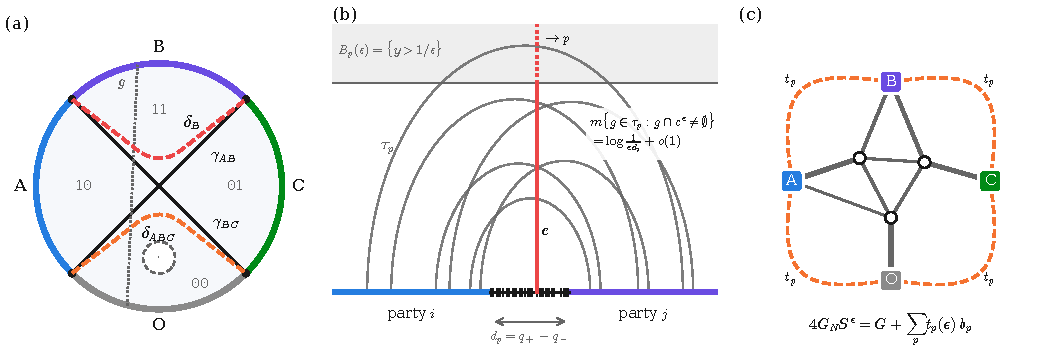
\includegraphics[width=\textwidth]{fig/fig2_mechanism.pdf}
\caption{(a)~Cut-and-paste on one arrangement (strong subadditivity; local picture on the quotient surface,
Klein model). Cells carry the bits $(x_{AB},x_{BC})$; the outputs $\delta_B$ and $\delta_{ABC}$ bound the cells
labelled $11$ and the cells $\neq00$, resolved at the vertex. Any geodesic $g$ crosses the inputs at least as
often as the outputs; integrating over $g$ with the measure $\mu$ gives the inequality for both chiral lengths
simultaneously. (b)~Chart with the entangling point $p$ at $\infty$. All other ideal points lie in
$[q_-,q_+]$. Geodesics of the class $\tau_p$ (gray) connect the two pieces adjacent to $p$; each crosses the cut
arc ending at $p$ (red) exactly once. Their mass up to the horoball is $\log(1/\eps d_p)+o(1)$, independent of
the cut. (c)~The resulting entropy vector: a finite graph whose min-cuts give the finite part $G$, plus one
edge of weight $t_p(\eps)$ (dashed) joining the parties adjacent at each entangling point.}
\label{fig:mechanism}
\end{figure*}

\emph{Renormalised Crofton formula and Bell pairs.}---%
For regions with endpoints the lengths diverge and $\mu$ has infinite mass. The divergence is concentrated in
a single topological class per endpoint. For $p\in P$, let $\tau_p$ be the class of geodesics connecting the
two boundary pieces adjacent to $p$ around $p$ [Fig.~\ref{fig:mechanism}(b)]. Every cut for $A$ crosses
every geodesic of $\tau_p$ exactly $e_p=[p\in\partial A]$ times, independently of the cut. In a chart with $p$ at
$\infty$ and cutoff horoball $\{y>1/\eps\}$, let $d_p$ be the length of the smallest interval containing all
other ideal points.

\begin{proposition}[Renormalised Crofton formula]\label{prop:crofton}
Let $m'_X$ be the Liouville measure of $X$ with the classes $\tau_p$ removed. Every class other than the
$\tau_p$ and those homotopic into the boundary has finite $m'_X$-mass, and for every cut class $c$ and
$\eps\le\eps_0$, exactly,
\begin{equation}\label{eq:crofton}
\ell^\eps_X(c)=\int i(g,c)\,dm'_X(g)+\sum_{p\in P}e_p(c)\,\log\frac{1}{\eps\,d_p}.
\end{equation}
\end{proposition}

The proof splits the Crofton integral into $\tau_p$ and the rest; the $\tau_p$ part is an explicit integral
whose value, $\log(1/\eps d_p)+o(1)$, does not depend on where the cut meets $p$, and the remainder converges
monotonically to the first term. Since $e_p(c)=[p\in\partial A]$ for every $c\in\Cut(A)$, Eqs.~\eqref{eq:H}
and~\eqref{eq:crofton} give, with $b_p(A):=[p\in\partial A]$,
\begin{equation}\label{eq:decomp}
\begin{aligned}
4G_N\,S^\eps&=G+\sum_{p\in P}t_p(\eps)\,b_p,\\
t_p(\eps)&=\log\frac1\eps-\frac12\log\big(d_p^Ld_p^R\big),
\end{aligned}
\end{equation}
where $G(A)=\min_{c\in\Cut(A)}i(\mu',c)$, $\mu'=\frac12(m'_L+m'_R)$, is independent of $\eps$. The vector $b_p$ is
the entropy vector of a Bell pair shared by the two parties adjacent at $p$ (the purifier included). With
$c=3/2G_N$, the Bell-pair weight is $t_p/4G_N=(c/6)\log(1/\eps)+O(1)$: \emph{the ultraviolet divergence of the HRT
entropies is exactly one Bell-pair term per entangling point}, carrying the universal $(c/6)\log(1/\eps)$ of
each endpoint, and everything else is a finite, cutoff-independent vector $G$. A change of cutoff scheme at $p$
shifts $t_p$ by a constant and $G$ by a multiple of $b_p$.

\emph{The cone.}---%
\begin{theorem}[Covariant entropies lie in the RT cone]\label{thm:main}
For every spacetime of the class above and every assignment of $N$ parties to intervals and whole boundaries:
\begin{enumerate}
\item[(i)] $G$ is the min-cut function of a finite weighted graph; hence $S^\eps\in\CN$ for all
$\eps\le\min(\eps_0,\eps_1)$, $\eps_1=\min_p(d_p^Ld_p^R)^{-1/2}$.
\item[(ii)] For every linear inequality $Q\ge0$ valid on $\CN$ and every $\eps\le\eps_0$,
$Q(4G_NS^\eps)=Q(G)+\sum_pt_p(\eps)\,Q(b_p)$, with $Q(G)\ge0$ and $Q(b_p)\ge0$. The slack is independent of $\eps$
if $Q$ is balanced at every entangling point, and diverges to $+\infty$ as $\eps\to0$ otherwise.
\end{enumerate}
\end{theorem}

The graph in (i) is explicit [Fig.~\ref{fig:mechanism}(c)]: draw minimisers of $G$ for all regions on $X_L$;
the vertices are the cells of this arrangement (each cell touching the boundary contains pieces of one party
only), and each segment of the arrangement gives an edge between the two adjacent cells, weighted by the
$\mu'$-mass of the geodesics crossing it. The minimiser for each region gives a vertex set whose cut weight is $G(A)$, and
conversely every admissible vertex set is resolved by the cut-and-paste step into a cut of no larger $\mu'$-mass.
This is the argument of Ref.~\cite{Bao2015} for static RT, run in the virtual geometry of $\mu'$; it requires
finite edge weights, which is why the endpoint classes must first be split off as Bell pairs. Adding an edge of
weight $t_p\ge0$ between the terminals adjacent at each $p$ realises $4G_NS^\eps$ itself.

No contraction map and no completeness claim about contraction maps~\cite{BaoFuruyaNaskar2025} is used, so (ii)
covers every facet of $\CN$, including the facet orbit of $\mathcal{C}_5$ that has no contraction map in
weighted form~\cite{AvisHernandezCuenca2023} and inequalities that are not superbalanced~\cite{JuCzech2026}.
For the latter, Eq.~\eqref{eq:decomp} locates the divergence: it comes from the entangling points between
parties $i,j$ with $Q(b_{ij})>0$.

\begin{theorem}[Cone equality]\label{thm:equality}
Let $\mathcal{H}_N$ be the set of vectors $4G_NS^\eps$ over all spacetimes of the class, all $N$-party
assignments and all $\eps$ below the threshold. Then $\overline{\mathbb{R}_{>0}\mathcal{H}_N}=\CN$; static
multiboundary wormholes with whole-boundary parties already suffice.
\end{theorem}

The inclusion $\subseteq$ is Theorem~\ref{thm:main}. For $\supseteq$, every graph model is realised, up to scale,
by the RT entropies of a hyperbolic surface glued from pairs of pants along geodesics of lengths proportional to
the edge weights~\cite{Bao2015}; that surface with $X_L=X_R$ is a static wormhole. For whole-boundary parties
the HRT vector of any rotating wormhole is therefore, up to a positive factor, the RT vector of a static
multiboundary wormhole.

\begin{figure}[t]
\centering
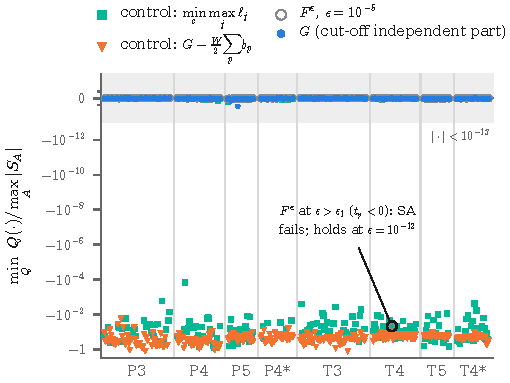
\includegraphics[width=\columnwidth]{fig/fig3_numerics.pdf}
\caption{Smallest facet value $\min_QQ(\cdot)/\max_A|S_A|$ of $\mathcal{C}_3,\mathcal{C}_4,\mathcal{C}_5$
(7, 20 and 372 facets) for 308 random configurations on pairs of pants (P) and one-holed tori (T) with two
metrics of common marking, $N=3,4,5$ parties (asterisk: wider parameter ranges). $G$ and $F^\eps$ lie at
rounding level; the single $F^\eps$ outlier has $\eps>\eps_1$ and is removed at smaller $\eps$, as
Theorem~\ref{thm:main}(i) predicts. Two control functionals violate facets in most configurations.}
\label{fig:numerics}
\end{figure}

\emph{Numerical tests.}---%
The proofs are analytic; numerics test conclusions only. On rank-two Schottky surfaces (three-holed spheres and
one-holed tori) with two independent metrics of common marking, random positive weights generalising
$w_L=w_R=\frac12$, $N=3$--$5$ parties and 2--7 marked points, we computed $F^\eps$ by exhaustive search over
embedded cuts with bounded word length (stable under increasing the length in all 102 rechecked
configurations), extracted $G$ from Eq.~\eqref{eq:decomp}, and evaluated all facets (Fig.~\ref{fig:numerics}).
Over 4428 regions, $G$ is $\eps$-independent to $2\times10^{-14}$ and satisfies every facet; the common-class
constraint changes the minimiser in 147 regions. Two controls---subtracting only half the endpoint terms, and
$\min_c\max_j\ell_j(c)$---violate facets in most configurations. On the disc, the explicit graph of
Theorem~\ref{thm:main}(i) reproduces $G$ to $5\times10^{-14}$, and on the cylinder Eq.~\eqref{eq:crofton}
holds to $6\times10^{-14}$~\cite{SM}.

\emph{Discussion.}---%
For three-dimensional vacuum gravity, covariant holographic entropies obey exactly the inequalities of the static
cone: the closure of the set of covariant entropy rays is the RT cone. The mechanism is that the HRT functional is
an RT functional for the virtual geometry of a single geodesic current on the quotient surface, and that the
ultraviolet divergence separates exactly into Bell pairs at the entangling points. The same decomposition makes
the UV structure of every valid inequality explicit. The novelty is the identification of the HRT entropy with
this functional for every cut class (Theorem~\ref{thm:H}), the topological contraction on the quotient, the
renormalised Crofton formula and the graph realisation; the pleated geometry~\cite{MazzoliViaggi2022}, the
correspondence between currents and pseudo-metrics~\cite{BIPP2021,MartinezGranadoThurston2026}, the extension
theorems~\cite{BernalSanchez2006,AkeFloresSanchez2021} and the realisation of graphs by static
wormholes~\cite{Bao2015} are prior work.

Vacuum enters only through positivity of $\mu$, which here is a sum of two Liouville measures. With matter
obeying the null energy condition, Czech and Dong obtain a positive measure from strong subadditivity on the
universal cover~\cite{CzechDong2019}; the missing step for multiply connected bulks is to turn it into a
$\pi_1$-invariant measure on the quotient whose integrals reproduce the lengths of closed extremal curves.
% MATTER-SLOT (discussion): replace the preceding two sentences by the statement of the matter result and its
% hypotheses if that extension is established.
In higher dimensions there is no chiral decomposition and extremal surfaces are not geodesics. Within $2+1$
dimensions, open cases are extremal horizons and conical defects, achronal homology slices with null
pieces~\cite{Wall2014}, prescriptions not requiring the homology region to lie on a Cauchy slice, and quantum
corrections. Complete proofs and the numerical methods are in the \SM.

\begin{acknowledgments}
[Acknowledgments placeholder.]
\end{acknowledgments}

\bibliographystyle{apsrev4-2}
\bibliography{refs}

\end{document}
